\documentclass[12pt, a4paper]{book}%, oneside

\usepackage[headings]{fullpage}
\usepackage{setspace}

% \usepackage[top=1.5cm,right=1.5cm,bottom=1.5cm,left=1.5cm]{geometry}
\usepackage{graphicx}
\usepackage{float}
\usepackage{subfig}
\usepackage{array}
\usepackage{multirow}
\usepackage{booktabs}
\usepackage{appendix}
\usepackage[pdfborder={0 0 0}, colorlinks=true, linkcolor=black, citecolor=blue]{hyperref}
\usepackage[printonlyused]{acronym}
\usepackage{algorithmic}
\usepackage{algorithm}
\usepackage{ifpdf}

\usepackage[utf8]{inputenc}

\newcommand{\keywords}{Brain Computer Interface, BCI, Machine Learning, ML, P-300, P-300 Speller, On-Screen Keyboard, Keyboard}

\newcommand{\submissionDay}{26}
\newcommand{\submissionMonth}{May}
\newcommand{\submissionYear}{2019}
\newcommand{\submissionDate}{\submissionDay~\submissionMonth,~\submissionYear}
\newcommand{\typeOfThesis}{Bachelor Thesis - Expository}

\newcommand{\titleOfThesisOne}{A Brain-controlled On-screen Assistive Keyboard}

\newcommand{\authorOfThesis}{Maqarios Wagdy Tawadros Saleh Mohareb}
\newcommand{\supervisor}{Assoc. Prof. Seif El-Dawlatly}

\newcommand{\includefig}[4]{
    \begin{figure}[ht]
     \centering
      \includegraphics[width=#1\textwidth]{images/#2}
      \caption{#3}
      \label{#4}
    \end{figure}
}

\newcommand{\includefigWSC}[5]{
    \begin{figure}[ht]
     \centering
      \includegraphics[width=#1\textwidth]{images/#2}
      \caption[#3]{#4}
      \label{#5}
    \end{figure}
}

\newcommand{\includeeps}[4]{
\includefig{#1}{#2.eps}{#3}{#4}
}

\newcommand{\includeepsWSC}[5]{
\includefigWSC{#1}{#2.eps}{#3}{#4}{#5}
}


\ifpdf
\pdfinfo {
	/Author (\authorOfThesis)
	/Title (\titleOfThesisOne)
	/Subject (\typeOfThesis)
	/Keywords (\keywords)
	/CreationDate (D:20090707085533)
}
\fi

\begin{document}
% \overfullrule=5pt
\pagestyle{plain}
\pagenumbering{Roman}

\newcommand{\titlePage}{

\thispagestyle{empty}
\begin{center}
	\textbf{Media Engineering and Technology Faculty}\\[1mm]
	\textbf{German University in Cairo}\\[1mm]
	
\includegraphics[width=2.5cm]{GUC-logo-ss.eps}
	
	\vspace{2cm}
	\doublespacing
	{\Huge \textbf{\titleOfThesisOne}}\\
	\singlespacing
	\vspace{2cm}
	{\large \textbf{\typeOfThesis}}\\
	
	\vfill
	\parbox{1cm}{
  		\begin{large}
    			\begin{tabbing}
       			Author: \hspace{2cm}  
        			\=\authorOfThesis\\[2mm]
      			Supervisors: 
        			\>\supervisor\\[2mm]
      			Submission Date: 
        			\>\submissionDate\\
    			\end{tabbing}
  		\end{large}
	}\\
\end{center}
\clearpage
}
%++++++++++++++++++++++++++++++++++++++++++++++++++++++++++++++++++++
\titlePage
\thispagestyle{empty}\ \clearpage
\titlePage
%++++++++++++++++++++++++++++++++++++++++++++++++++++++++++++++++++++
\thispagestyle{empty}
This is to certify that:
\begin{itemize}
\item[(i)] the thesis comprises only my original work toward the Bachelor Degree
\item[(ii)] due acknowlegement has been made in the text to all other material used
\end{itemize}

\vspace{2cm}
\begin{flushright}
\rule[0mm]{6cm}{0.2mm}\\
\authorOfThesis\\
\submissionDay~\submissionMonth,~\submissionYear\\
\end{flushright}
\clearpage


\chapter*{Acknowledgments}\label{chap:acknowledgments}

\paragraph{}
First of all, I would like to express my at-most gratitude to my supervisor Assoc. Prof. Seif El-Dawlatly for his support and immense knowledge. His sincere guidance helped me a lot in the time of research, application, experimentation and writing of this thesis.

\paragraph{}
Besides my supervisor, I thank my colleagues Ahmed Alaa, Mostafa Nasr and Omar Ashraf for giving me insightful arguments and collection of data.

\paragraph{}
Last but not least, I would like to thank my parents for the continuous support and patience.

\chapter*{Abstract}
\label{chap:abstract}
% ================================================================
In this project, an on-screen keyboard will be made. The main aim of this project is to help people with physical disability use computers more easily.\par
% ----------------------------------------------------------------
Using \ac{p300} based \ac{bci} which uses oddball paradigm to determine the required actions to be done by the application. By displaying a matrix of characters, the user can determine the character he wants from this matrix.\par
% ----------------------------------------------------------------
By processing the recorded brain waves to \ac{ml} model and apply mathematical filters to accurately determine the intended actions. Thus, reaching an accuracy with an average of 80\% in character recognition rate which is not bad compared to previous results obtained by previous papers \cite{inproceedings1, inproceedings2, article1, article2}.\par
% ----------------------------------------------------------------
\clearpage
% ================================================================
\tableofcontents
% \addcontentsline{toc}{chapter}{Contents}
\clearpage 

\pagestyle{headings}
\pagenumbering{arabic}

\setlength\parskip{.5\baselineskip plus .2\baselineskip
	minus .4\baselineskip}


\subsubsection{Motivation}
Imagine that one day, while you are setting on the bed too lazy to move. with this project all you need to do, is just one glance at the computer screen near you to send an email to your employer telling him that you are not coming today. Or having a disabled friend but wants to learn programming. all of these are possible using brain waves, In a parallel world brain waves is a synonyms for laziness.
\subsubsection{Objective}
The aim of this project is to build on-screen keyboard however without using clicks but brain waves to choose a character within a matrix.
\subsubsection{Brief Description}
A matrix of characters (i.e. 6x6) each cell has a character. The matrix is displayed for a certain period then each row and column will be intensified for a certain period of time randomly. The row and column which has a certain wave form is their intersection is the chosen character.
\section{Introductory to BCIs}
BCI Stands for (Brain-Computer Interface) which refers to intercepting the brain waves through some means such as electrodes, which is then transmitted to a computer after amplifying and digitizing the signal (Figure 2.1). The process starts with the intent of the user to do some action such as raising the right hand, the BCI records the brain activity and sends the intercepted signals to the BCI applications to do the desired reaction. There are several terms such as BMI (Brain-Machine Interface) or DBI (Direct Brain Interface) have the same meaning as BCI, however there are some terms such as Neuroprosthesis are not the same because BCI refers to only receiving (intercepting) data from the brain, however Neuroprosthesis refers to both sending and receiving data to and from the brain. In other words, BCI is a subset of Neuroprosthesis.
\begin{figure}
    \centering
    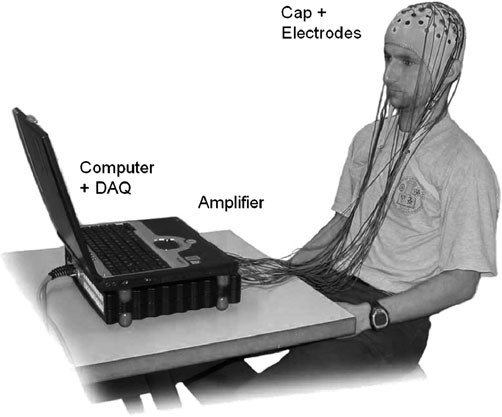
\includegraphics[width=70mm]{images/figure-2-1.jpg}
    \caption{Person records BCI data}
    \label{fig:my_label}
\end{figure}


\subsection{Processes of Operation}
BCI goes through three main procedures, measuring the brain activity, processing it and controlling the intercepted signals.
\subsubsection{Measuring Brain Activity}
Brain activity produces magnetic and electrical waves. That’s why, sensors or electrodes are used to measure these changes at different areas and times. Brain activities can be recorded through sensors (non-surgical solution) or electrodes (surgical solutions). For the non-surgical solution, sensors are used to measure the electrical activity from the scalp and this solution is called Electroencephalography (EEG) (Figure 2.1). They are relatively easy to deal with however they don’t provide accurate measures due to external interference and are susceptible to limitations in frequency range. In order to get consistent recording, sensors are spread on the scalp through system called 10 - 20 (Figure 2.2). 10 - 20 refers to how sensors are spread 10 - 20 - 20 - 20 - 20 - 10 percent. The 6 regions are named according to their position: Fp - pre-frontal, F - frontal, C - central, P - parietal, O - occipital, T - temporal. On the other hand, the surgical solution need to open the skull through surgical procedures and plant the electrodes. When the electrodes are planted on the surface of the cortex, it’s called electrocorticogram (ECoG). And another solution called Intracortical, which plants the electrodes in the inner parts of the brain. Although the surgical solutions provide higher accuracy and frequency range compared to the non-surgical solution they have serious drawbacks such as they need surgery, finance and can have ethical problems. Difference between each solution is shown in Figure 2.3.
\begin{figure}
    \centering
    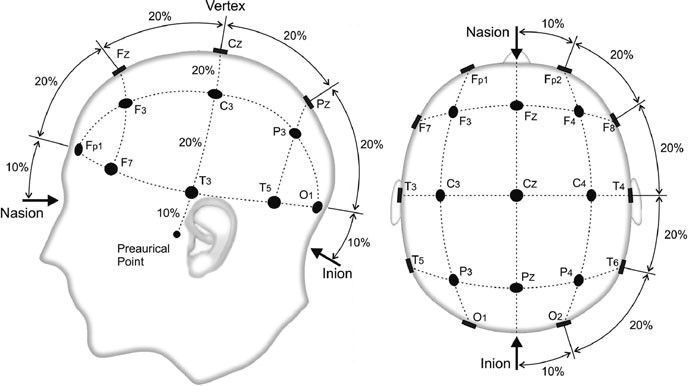
\includegraphics[width=70mm]{images/figure-2-2.jpg}
    \caption{10 - 20 System that shows how sensors are spread on the scalp}
    \label{fig:my_label}
\end{figure}
\begin{figure}
    \centering
    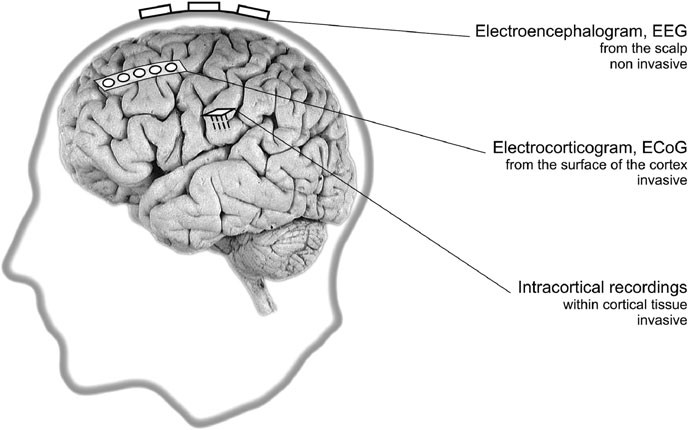
\includegraphics[width=70mm]{images/figure-2-3.jpg}
    \caption{Types of Reading Brain Waves on Computers (BCIs)}
    \label{fig:my_label}
\end{figure}

\subsubsection{Process and Control}
Processing and Controlling Received Signals are handled within the application.

\subsection{Brain Patterns}
Because measuring brain activity is not enough, some mental strategies are used to trigger the required tasks. The most used mental strategies are selective attention and motor imagery.
\subsubsection{Selective Attention}
Mental strategies based on selective attention require external stimuli such as auditory stimuli or visual stimuli. P300 (Peak signal at 300ms) or SSVEP (Steady-State Visual Evoked Potentials) are two mental strategies the depends on visual stimulation. P300 is triggered when the intensity of symbols is changed and SSVEP is triggered with flickering some areas with certain frequencies (6 – 30Hz).


\section{Online Dataset}
BCI2000, Competition III, Dataset II.

\subsection{Paradigm}
The user was shown a 6 by 6 matrix containing English letters and numbers (Figure 2.4). The user was to spell words and focus his attention of the character that he wants to choose. All rows and columns were intensified randomly and successively at a rate of 5.7Hz (100ms intensification, 75ms no intensification). In other words, a column or row is intensified (i.e. row 2 in Figure 2.4) for 100ms then, no row or column is intensified for 75ms, then repeat. The row and column (2 intensifications) which contained the chosen character will provide different signals (P300) compared to the other 10 intensifications which does not contain the chosen character (Non-P300).
\begin{figure}
    \centering
    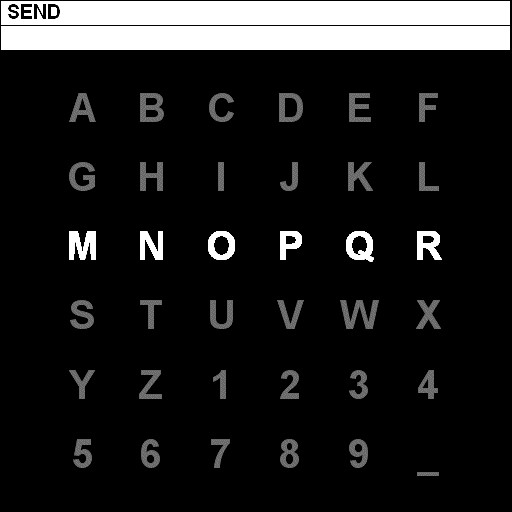
\includegraphics[width=70mm]{images/figure-2-4.jpg}
    \caption{The matrix displayed to the user}
    \label{fig:my_label}
\end{figure}

\subsection{Collection of Dataset}
Signals are filtered from 0.1 – 60Hz and digitized at 240Hz (Each 240 samples corresponds to 1 second). The 12 sets of intensifications were repeated 15 times for each character resulting in 180 total intensifications per epoch (character) into 64 channels EEG (Figure 2.5).
\begin{figure}
    \centering
    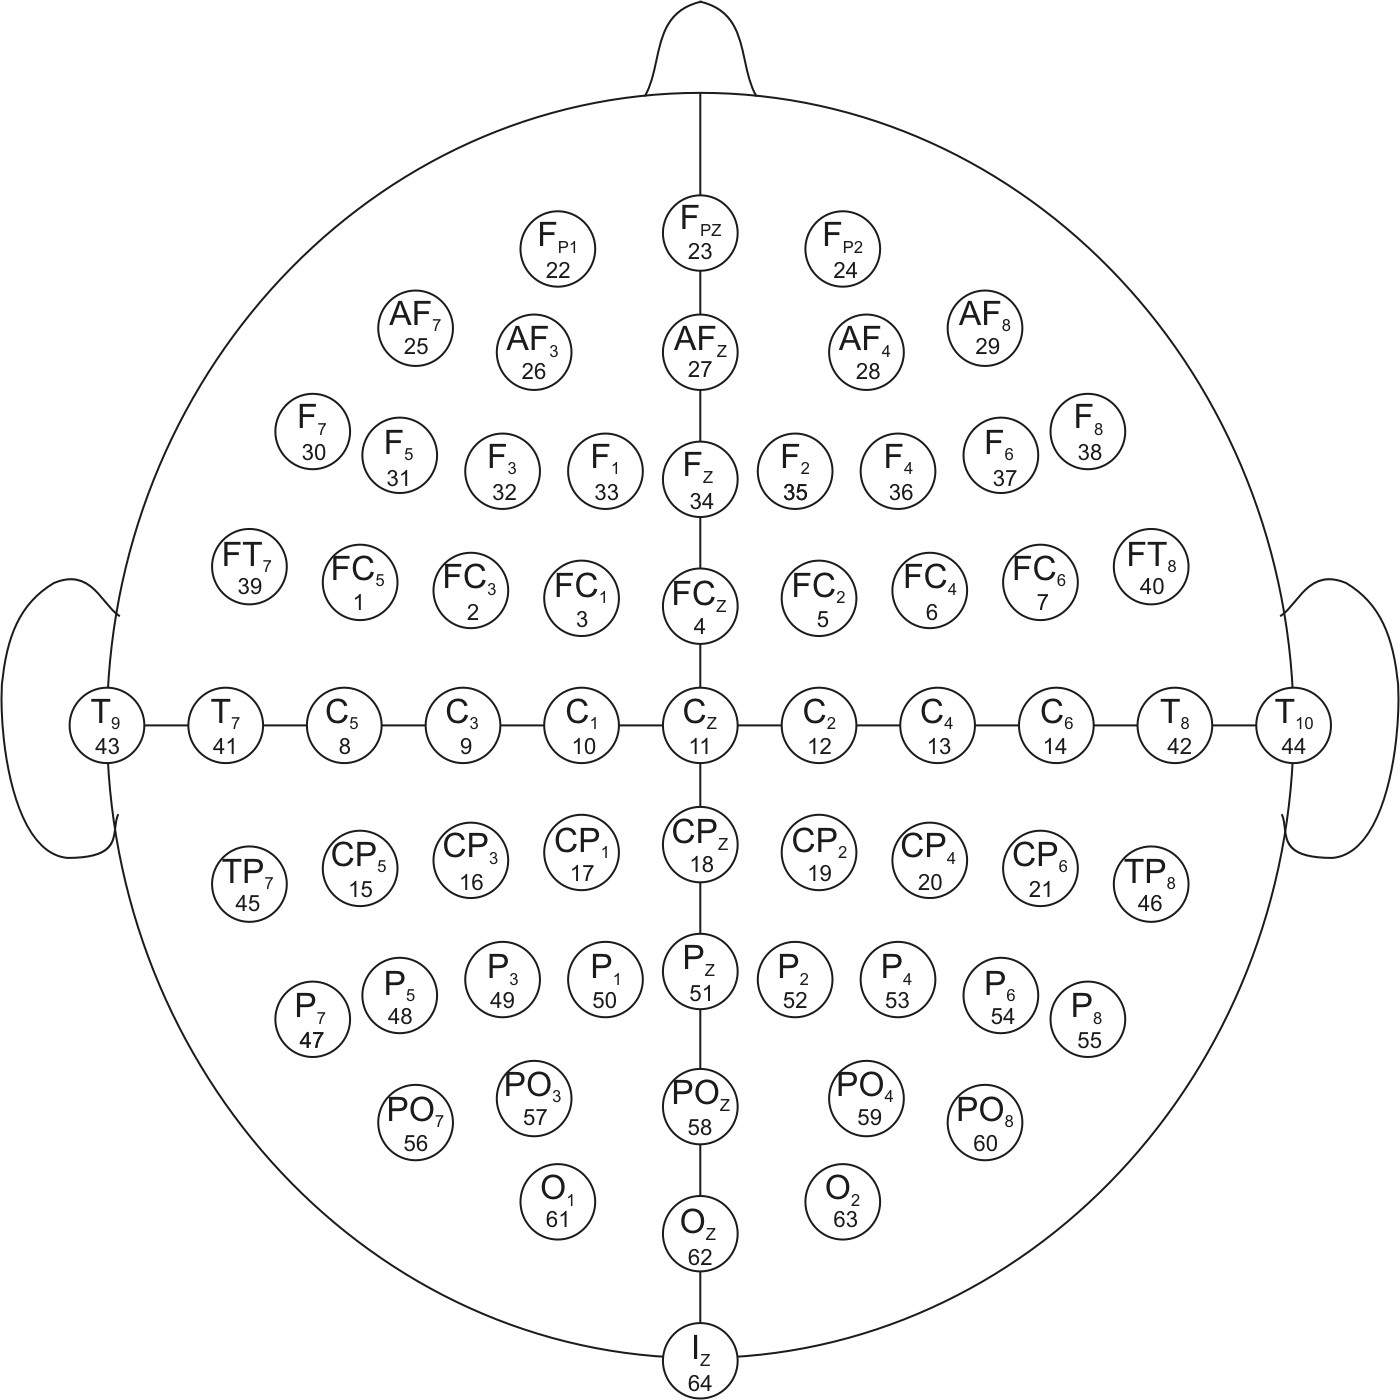
\includegraphics[width=70mm]{images/figure-2-5.jpg}
    \caption{Mapping of each sensors to its place on the scalp}
    \label{fig:my_label}
\end{figure}

\subsection{Explanation of The Dataset}
The dataset has 2 subjects (A and B), where each subject has 85 characters (epochs) in training dataset and 100 characters in testing dataset (Remember that, each epoch has 12 intensifications and 15 repetitions). The structure of variables for each subject file is described below.\newline
\begin{tabbing}
Title:\quad \quad \quad \quad \quad \=Description\kill
Signal:         \>signal of each channel (Figure 2.5)\\
                \>Type: 3D Array\\
                \>Shape (Dimension): (85, 7794, 64)\\
\newline\\
TargetChar:     \>The chosen character for each epoch\\
                \>Type: String\\
                \>Length: 85\\
\newline\\
Flashing:	    \>0	when NO row/column is intensified\\
                \>1	when row/column is intensified\\
                \>Type: 2D Array\\
                \>Shape (Dimension): (85, 7794)\\
\newline\\
StimulusCode:	\>0	when NO row/column is intensified\\
                \>1 ... 6	when intensified column (1 is left-most column)\\
                \>7 ... 12	when intensified row (1 is upper-most row)\\
                \>Type: 2D Array\\
                \>Shape (Dimension): (85, 7794)\\
\newline\\
StimulusType:	\>0	when NO row/column is intensified\\
		        \>1	when row/column contains the chosen character\\
                \>Type: 2D Array\\
                \>Shape (Dimension): (85, 7794)\\
\end{tabbing}
Note: 7794 samples because the data is digitized and there is a no-intensification period between each intensification.
Note: TargetChar, StimulusType are only provided for training dataset.

\subsection{Analysis}
Figure 2.6 shows signal wave forms for P300.
\begin{figure}
    \centering
    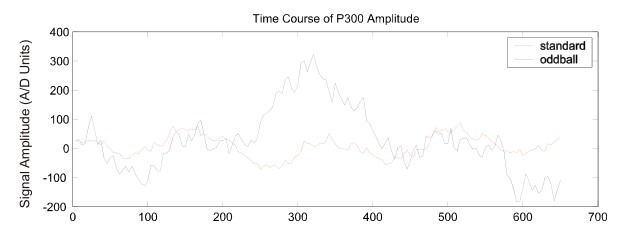
\includegraphics[width=70mm]{images/figure-2-6.jpg}
    \caption{Caption}
    \label{fig:my_label}
\end{figure}



\chapter{Conclusion and Future Work}
\label{chap:conclusion}
% ================================================================
\section{Conclusion}
In conclusion, using \ac{p300} based \ac{bci} a \ac{p300} speller was programmed. Using \ac{ml} and specifically \ac{lda} classifier, a character recognition rate of around 80\% in the competition's dataset and 70\% in the recorded dataset was achieved. The number of channels didn't have much effect, at least it depends on the subject, their brain waves and their state of mind \ref{tab:subject-A-B-char-reco}.\par
% ----------------------------------------------------------------
However, one could see that applying filters did have great impact on the character recognition rate. As shown in Table \ref{tab:subject-C-D-char-reco}, an increase of around 20\% was achieved on subject C, however, on subject D there was no effect at all, mainly due to signal interference, lack of attention and lack of experience with the platform. One can see that effect from the \ac{p300} plot in Figure \ref{fig:subject-C-p300} versus Figure \ref{fig:subject-D-p300}.\par
% ----------------------------------------------------------------

\section{Future Work}
There is a lot can be done to increase the efficiency of this project. Such as trying different combinations of filters and classifiers for each subject since \ac{ml} models are like maths problems where one can achieve the desired answer with more than one way.\par
% ----------------------------------------------------------------
An auto-complete functionality can be added as well in order to save time. one character takes around 30 seconds to be determined. If we consider the average of one word to be 5 characters, then, this will take around 150 seconds in total which is a lot for one word. However, if auto-complete was added it can take half the time to determine what the user wants thus saving a lot of time.\par
% ----------------------------------------------------------------
Sentence's prediction and adaptability can be added as well. As it can check what the user tends to type so often then add it as a shortcut instead of typing the whole sentence from the beginning and predicting next word within the current sentence (same behavior as mobile keyboards).\par
% ----------------------------------------------------------------
A mobile phone application can be programmed as well since \ac{p300} speller does not require much computation. However, it will be hard to do it on mobile phones with small screens or older version platforms since it might not be compatible with the headset.

\clearpage
% ================================================================
\chapter{Future Work}\label{chap:future_work}
text
\appendix
\renewcommand{\appendixtocname}{Appendix}
\renewcommand{\appendixpagename}{\appendixtocname}
\addappheadtotoc
\setboolean{@twoside}{false}
\appendixpage

\chapter{Lists}
\addcontentsline{toc}{section}{List of Abbreviations}
\begin{acronym}[\hspace{3cm}]
    \acro{bci}[BCI]{Brain–Computer Interface \cite{inbook1}}
    \acro{bmi}[BMI]{Brain-Machine Interface}
    \acro{car}[CAR]{Common Average Reference \cite{inproceedings1, inproceedings2, article2}}
    \acro{dbi}[DBI]{Direct Brain Interface}
    \acro{decimation}{Decimation \cite{inproceedings1, inproceedings2, article1, article2}}
    \acro{ecog}[ECoG]{Electrocorticogram \cite{inbook1}}
    \acro{eeg}[EEG]{Electroencephalography \cite{inbook1}}
    \acro{erp}[ERP]{Event Related Potential}
    \acro{gui}[GUI]{Graphical User Interface}
    \acro{icr}[ICR]{Intracortical Recordings \cite{inbook1}}
    \acro{lda}[LDA]{Linear Discriminant Analysis}
    \acro{ma}{Moving Average \cite{inproceedings1, inproceedings2, article1}}
    \acro{ml}[ML]{Machine Learning \cite{article7}}
    \acro{p300}[P300]{Peak 300 \cite{article3}}
    \acro{sci}[SCI]{Spinal Cord Injury}
    \acro{ssvep}[SSVEP]{Steady State Visually Evoked Potential
    \cite{article4}}
    \acro{zscore}{Z-Score \cite{inproceedings1, article2}}
\end{acronym}
\clearpage


\listoffigures
\addcontentsline{toc}{section}{List of Figures}
\clearpage


\listoftables
\addcontentsline{toc}{section}{List of Tables}
\clearpage


%\listofalgorithms
%\addcontentsline{toc}{section}{List of Algorithms}
%\clearpage

\bibliographystyle{plain}
\bibliography{bachelor}
\addcontentsline{toc}{chapter}{References}

\end{document}
